
\chapter{Implementacja}

\section{REST API}
REST API jest to interfejs służący do komunikacji między Backendem i Frontendem, przez to realizując architekturę klient-serwer. W naszym projekcie został zaimplementowany 
za pomocą frameworka Spring Boot. Dzięki niemu możliwa była wydajna i prosta integracja z bazą danych PostgreSQL, która jest istotnym
punktem naszego systemu. Użycie Spring Boota umożliwiło zastosowanie operacji CRUD, które z kolei są możliwe do implementacji dzięki 
metodom HTTP takim jak: GET, PUT, POST, DELETE. Ważna cecha jaką jest warstwowość pozwoliła nam na oddzielenie części aplikacji:
\begin{itemize}
    \item Warstwa prezencji - składa się z kontrolerów, z których zarówno może korzystać frontend oraz inne serwisy.
    \item Warstwa serwisowa - składająca się z serwisów, które odpowiadają za logikę biznesową aplikacji.
    \item Warstwa dostępu do danych - składają się z repozytoriów, które odpowiadają za operacje na bazie danych.
    \item Warstwa infastrukturalna - składająca się z wielu komponentów, odpowiedzialnych głównie za konfigurację oraz kontakt z zewnętrznymi
    serwisami.
\end{itemize}

Wszystkie endpointy zabezpieczone są za pomocą tokenów JWT, dzięki czemu unikamy nieautoryzowanego dostępu do danych. 

Poszczególne błędy walidacyjne, lub z warstwy serwisowej oraz bazodanowej, wychwytywane są przez dedykowane handlery, które zapewniają ustandaryzowaną odpowiedź w formacie JSON wraz z
odpowiednim kodem statusu HTTP. 

Dla endpointów z potencjałem na zwracanie bardzo dużej ilości danych dodaliśmy mechanizm paginowania. Odpowiedzi dzielone są na strony 
co znacznie usprawnia wydajność przesyłania danych.

\begin{figure}[h!]
    \centering
    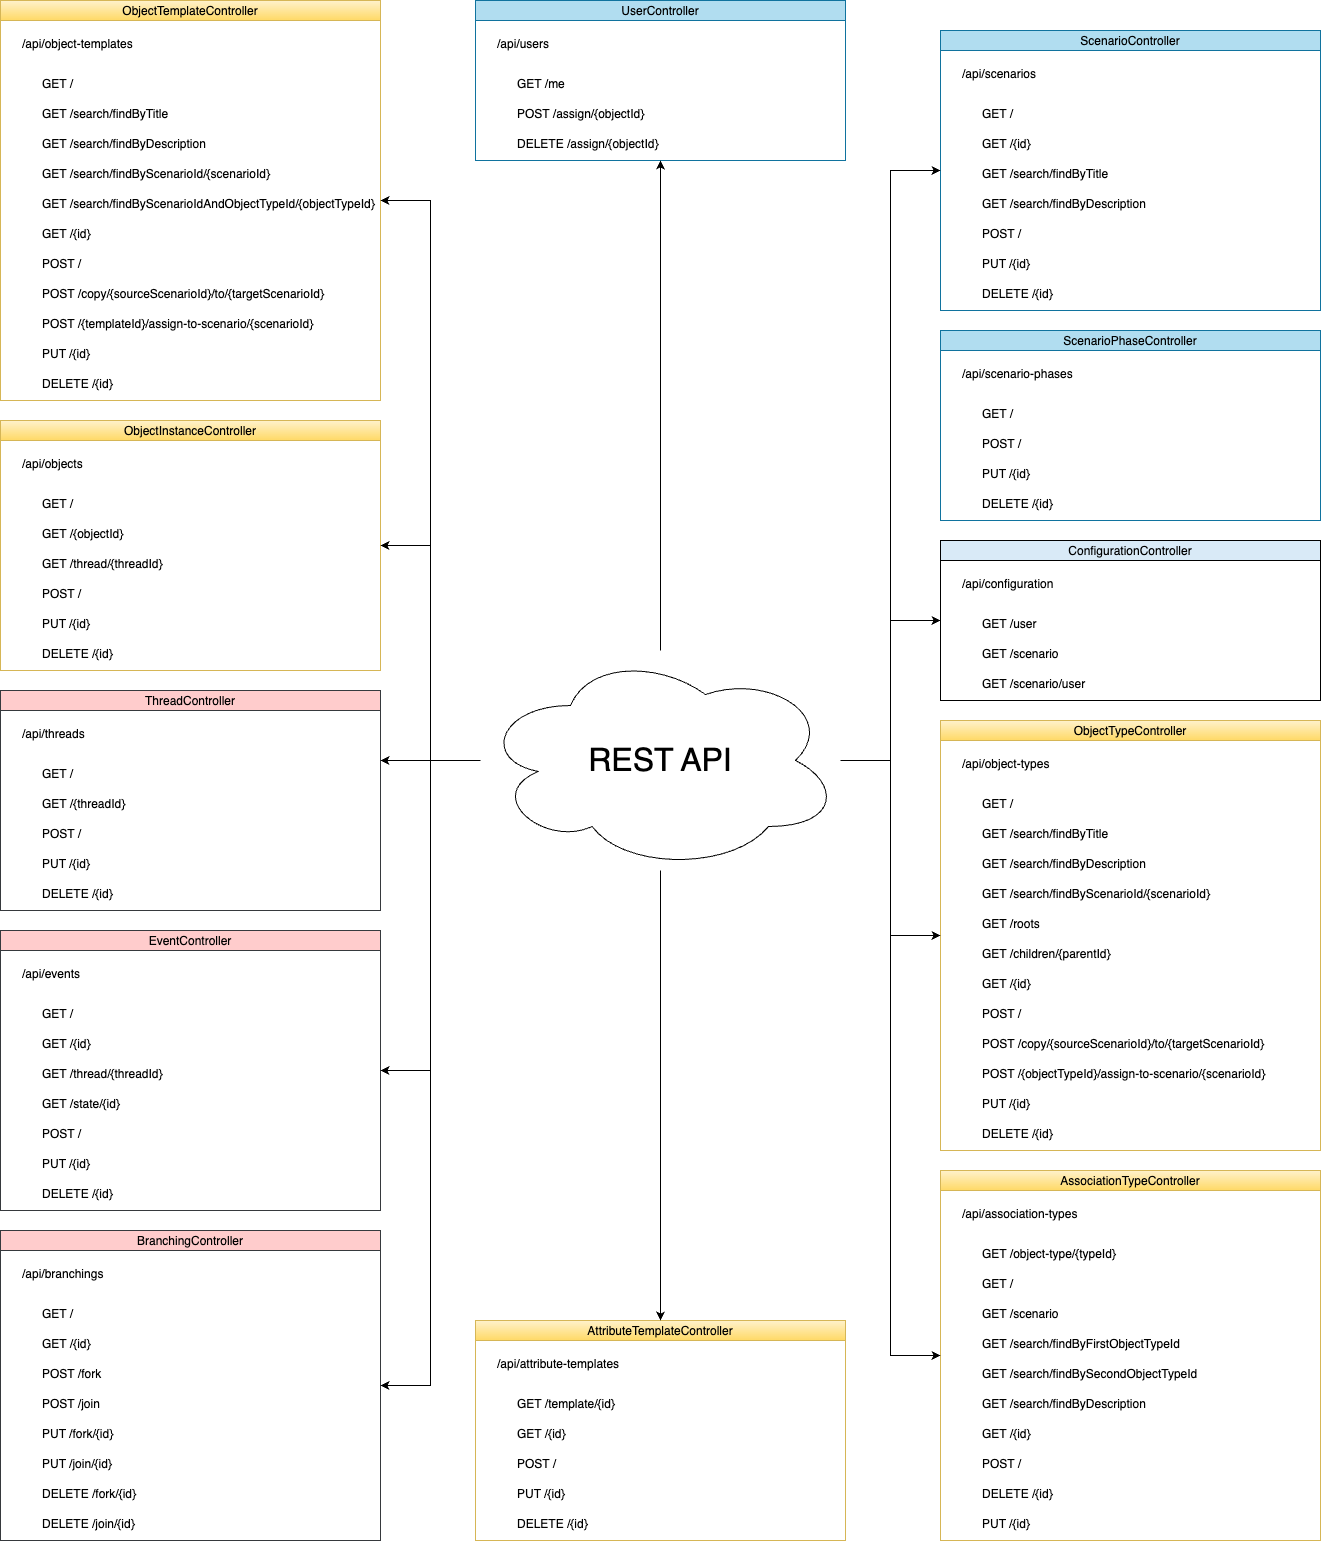
\includegraphics[width=0.99\textwidth]{resources/local/diagram-api.png}
    \caption{Diagram REST API}
\end{figure}

\section{Backend}

\subsection{Autoryzacja oraz uprawnienia}

Autoryzacja w naszej aplikacji obejmuje wszystkie endpointy, z wyjątkiem tych zdefiniowanych w liście odstępstw:
\begin{itemize}
    \item Autoryzacja i zdarzenia z keycloacka,
    \item Dokumentacja,
    \item Monitorowanie stanu aplikacji.
\end{itemize}
Odbywa się ona za pomocą tokenów JWT. Znajduje się on w kontekście bezpieczeństwa danego requesta, w obiekcie Authentication.
Dzięki danym znajdującym się w tokenie oraz wymaganym nagłówku posiadającym id scenariusza możemy sprawdzić czy użytkownik posiada uprawnienia edycji 
lub modyfikacji konkretnego scenariusza. Ważnym elementem architektury bezpieczeństwa naszej aplikacji jest CORS. 
Zablokuje on jakiekolwiek połączenia z niezdefiniowanych przez nas domen. Znacznie zwiększa to bezpieczeństwo aplikacji. 
w konfiguracja CORS-a definiujemy akceptowalne domeny, metody HTTP oraz nagłówki. W konfiguracji określamy także, że 
nie tworzymy oraz utrzymuje sesji HTTP dla użytkowników, ponieważ nie jest to potrzebne w sytuacji gdy wykorzystujemy mechanizm
tokenów. Za każdym razem posiadamy potrzebne dane autoryzacyjne. Wyłączamy także ochronę przed atakiem CSRF, która to jest domyślnie 
ustawiona w Spring Boot. Taki atak nie jest zagrożeniem w naszej polityce zarządzania sesjami.

Zdefiniowanie oddzielnych profili: deweloperskiego oraz produkcyjnego, pozwoliło nam na złagodzenie wielu warunków autoryzacyjnych
w sytuacji lokalnego uruchomienia aplikacji. 

\subsection{Obsługa błędów}

Błędy zwracane przez aplikację backendową wyglądają w następujący sposób:

\begin{lstlisting}[language=Java]
{
  "errorCode": "PHASE_OVERLAP",
  "errorGroup": "SCENARIO_PHASE",
  "values": ["12345"]
}
\end{lstlisting}

Wyjaśnienie poszczególnych części zwracanych błędów:
\begin{itemize}
    \item errorCode - klasa enum (wyliczeniowa), która zawiera w sobie szczegółowy kod błędu. Możemy ją potraktować jako
    ustandaryzowaną wiadomość wyjątku.
    \item errorGroup - klasa enum (wyliczeniowa), która mówi o tym z jaką częścią zapytania jest problem. Najczęściej odnosi się
    do konkretnej encji w bazie danych z nielicznymi wyjątkami.
    \item values - opcjonalna lista wartości kontekstowych, które można załączyć do błedu np. id obiektu w bazie. Ułatwia detekcje 
    problematycznego elementu.
\end{itemize}

W aplikacji posiadamy handlery, które odpowiadają za wychwytywanie błędów i transformowanie ich do jednolitej formy.
Możemy wyróżnić następujące typy handlerów:
\begin{itemize}
    \item bazodanowe - wychwytywanie błędów z bazy danych. Dopasowywujemy error code oraz error group na podstawie wiadomości wyjątku. Gdy dopasowanie nie
    jest możliwe zwracamy błąd serwera.
    \item walidacyjne - wychwytywanie błędów wynikających z błednych lub brakujących danych w requeście.
    \item biznesowe - wychwytywanie błędów rzucanych w warstwie biznesowej.
\end{itemize}

\subsection{Repozytoria}

Warstwa dostępu do danych, w naszej aplikacji, realizowana jest za pomocą repozytoriów JPA (Java Persistence API) dla poszczególnych encji. 
Takie podejście zapewnia gotowe funkcje CRUD, wspiera transakcje oraz umożliwia prostą implementację sortowania oraz paginacji.
Dla bardziej zaawansowanych zapytań stosujemy zapytania SQL. Pozwala nam na zejście z wysokiego poziomu abstrakcji, i operowanie
bezpośrednio na bazie danych.

\subsection{Walidacja danych}

Walidacja w naszym projekcie odbywa się na trzech warstwach: na poziome żądań, w logice biznesowej oraz bazie danych.
Pierwszy typ walidowania danych żądania realizujemy poprzez użycie biblioteki Jakarta Bean Validation. Umożliwia ona w prosty
i czytelny sposób oznaczać poszczególne atrybuty żądania za pomocą adnotacji. Przykładowy kod wykorzystujący tę bibliotekę
wygląda w następujący sposób:

\begin{lstlisting}[language=Java]
public record EventUpdateRequest(
  @NotNull(message = "NULL_VALUE;EVENT;description") String description,
  @NotNull(message = "NULL_VALUE;EVENT;title") String title,
  @NotNull(message = "NULL_VALUE;EVENT;associationChanges")
  @Valid
  List<AssociationChangeData> associationChanges,
  @NotNull(message = "NULL_VALUE;EVENT;attributeChanges")
  @Valid
  List<AttributeChangeData> attributeChanges
) {}
\end{lstlisting}

Jak widać w ukazanym kodzie adnotacja składa się z warunku, oraz wiadomości błędu zwracanej gdy dany wymaganie nie zostanie 
spełnione. Ponadto, dzięki użyciu adnotacji @Valid w stosunku do złożonych obiektów umożliwiamy hierarchiczną walidację.
Kolejnym istotnym aspektem jest użycie recordów, jako rodzaj klasy za pomocą której reprezentujemy dane wejściowe. Jest to stosunkowo
nowa funkcjonalność w języku Java, która ma na celu realizować rolę prostego nośnika danych. Ich główne zalety to:
\begin{itemize}
    \item Minimalizacja kodu,
    \item Niemutowalność,
    \item Poprawa czytelności kodu.
\end{itemize}

Do drugiego typu walidacji żądania wymagane są istniejące dane z bazy danych. Dobrym przykładem takiej walidacji jest transfer 
obiektów podczas rozdziału wątków. Musimy sprawdzić czy wszystkie obiekty zostały przeniesione do nowo utworzonych wątków, oraz 
czy obiekty związane razem asocjacją znajdują się w tym samym wątku. Za tego typu walidacje odpowiadają przeznaczone serwisy.

Ostatnim etapem walidacji żądania jest baza danych. W tym etapie wychwytywane są błędy zgłaszane przez bazę danych, oraz zmienianie
na wewnętrzny model błędu. Przykładowymi wyłapywanymi błędami z bazy danych są: brak klucza obcego, wartość NULL w kolumnie oznaczonej
jako NOT NULL lub naruszenie klucza obcego podczas usuwania obiektu. 

\subsection{Websocket}

Todo: napisać jak osiągnie ostateczną wersję

\subsection{Testy}

W aplikacji zaimplementowane zostały testy integracyjne oraz jednostkowe. Obydwa typy testów posiadają swoją bazową klasę
konfiguracyjną, która odpowiada za stworzenie bazy danych przy pomocy Testcontainers oraz wstrzyknięcie zależności przydatnych
w większości testów. Przykładem takiej zależności jest MockMvc, który umożliwia symulowanie żądań HTTP do kontrolerów.

Pokrycie endpointów testami wynosi 90\%. Dla nieprzetestowanych endpointów lepsze zastosowanie miały testy jednostkowe z powodu
skomplikowanej logiki biznesowej. Dla endpointów GET sprawdzany jest cały response za pomocą pliku JSON z poprawną odpowiedzią.
Pozostałe endpointy testujemy za pomocą asercji dotyczących stanu bazy danych.

\section{Frontend}
\subsection{Opis}
\subsubsection{Architektura systemu}
Interfejs użytkownika został opracowany w systemie Figma, na podstawie którego powstała aplikacja kliencka wykorzystująca TypeScript wraz z biblioteką React.js jako bazę interfejsu użytkownika.
\subsubsection{Warstwa wizualna i dostępność}
Warstwa wizualna opiera się na bibliotece Radix UI, dostarczającej komponenty typu headless\footnote{Komponenty headless to elementy interfejsu użytkownika pozbawione własnej warstwy prezentacji, dostarczające wyłącznie logikę działania i zachowania.}. Komponenty zaimplementowano przy użyciu biblioteki shadcn/ui, która dostarcza wzorce implementacji rozwiązań Radix UI do modyfikacji pod potrzeby zastosowań. Do stylizacji wykorzystano framework TailwindCSS. System dostosowuje interfejs do urządzeń mobilnych oraz stacjonarnych, zachowując standardy WCAG oraz wsparcie dostępności.

\subsubsection{Nawigacja i struktura aplikacji}
Panel boczny stanowi główny element nawigacyjny, adaptujący zawartość do kontekstu aplikacji. W katalogu scenariuszy zawiera nawigację wraz z listą ostatnio używanych scenariuszy. Panel zarządzania kontem znajduje się w dolnej części interfejsu.
Stan aplikacji oraz wyświetlanie paneli przechowywane są w parametrach URL\footnote{Część adresu URL po znaku zapytania, pozwalająca na przechowywanie stanu aplikacji w sposób umożliwiający nawigację przy użyciu funkcji przeglądarki}. Zapewnia to integrację z mechanizmami nawigacji przeglądarki.
\subsubsection{System powiadomień i obsługi błędów}
System powiadomień informuje użytkownika o statusie operacji API, błędach oraz ostrzeżeniach. Akcje użytkownika wyświetlają wskaźniki stanu ładowania. System obsługi błędów wznawia nieudane operacje API.

\subsubsection{Mechanizmy interakcji}
Aplikacja wykorzystuje nawigację klawiaturową oraz skróty klawiszowe dla wykonywanych akcji. Skróty obejmują dostęp do wyszukiwarki, nawigację po formularzach oraz operacje w edytorze scenariuszy. Elementy interakcji, przyciski akcji, formularze z walidacją oraz menu kontekstowe zachowują spójne działanie.
Formularze dialogowe wyposażone są w przycisk rozwijania zawartości w prawym górnym rogu. W trybie zwiniętym, pola posiadające dodatkowe informacje oznaczone są ikoną znaku zapytania. Po najechaniu kursorem na ikonę wyświetlana jest podpowiedź dotycząca danego pola. W trybie rozwiniętym, opisy pól prezentowane są w formie tekstu po lewej stronie formularza.

\subsubsection{Integracja z systemem}
Aplikacja wykorzystuje bibliotekę Keycloak.js do zarządzania stanem autoryzacji i komunikacji z serwerem uwierzytelniania. System działa jako oddzielna usługa, przekazując dane użytkownika. Dostęp do elementów aplikacji wymaga autoryzacji przez ten system.


Aplikacja używa interfejsu REST opisanego systemu backendowego. Do zarządzania stanem danych z API wykorzystano bibliotekę TanStack Query.

\subsection{Katalog scenariuszy}

Katalog scenariuszy stanowi główną stronę aplikacji, na którą następuje przekierowanie po autoryzacji. Z poziomu panelu bocznego dostępny jest katalog obiektów biblioteki oraz lista ostatnio edytowanych scenariuszy.

\begin{figure}[h]
    \centering
    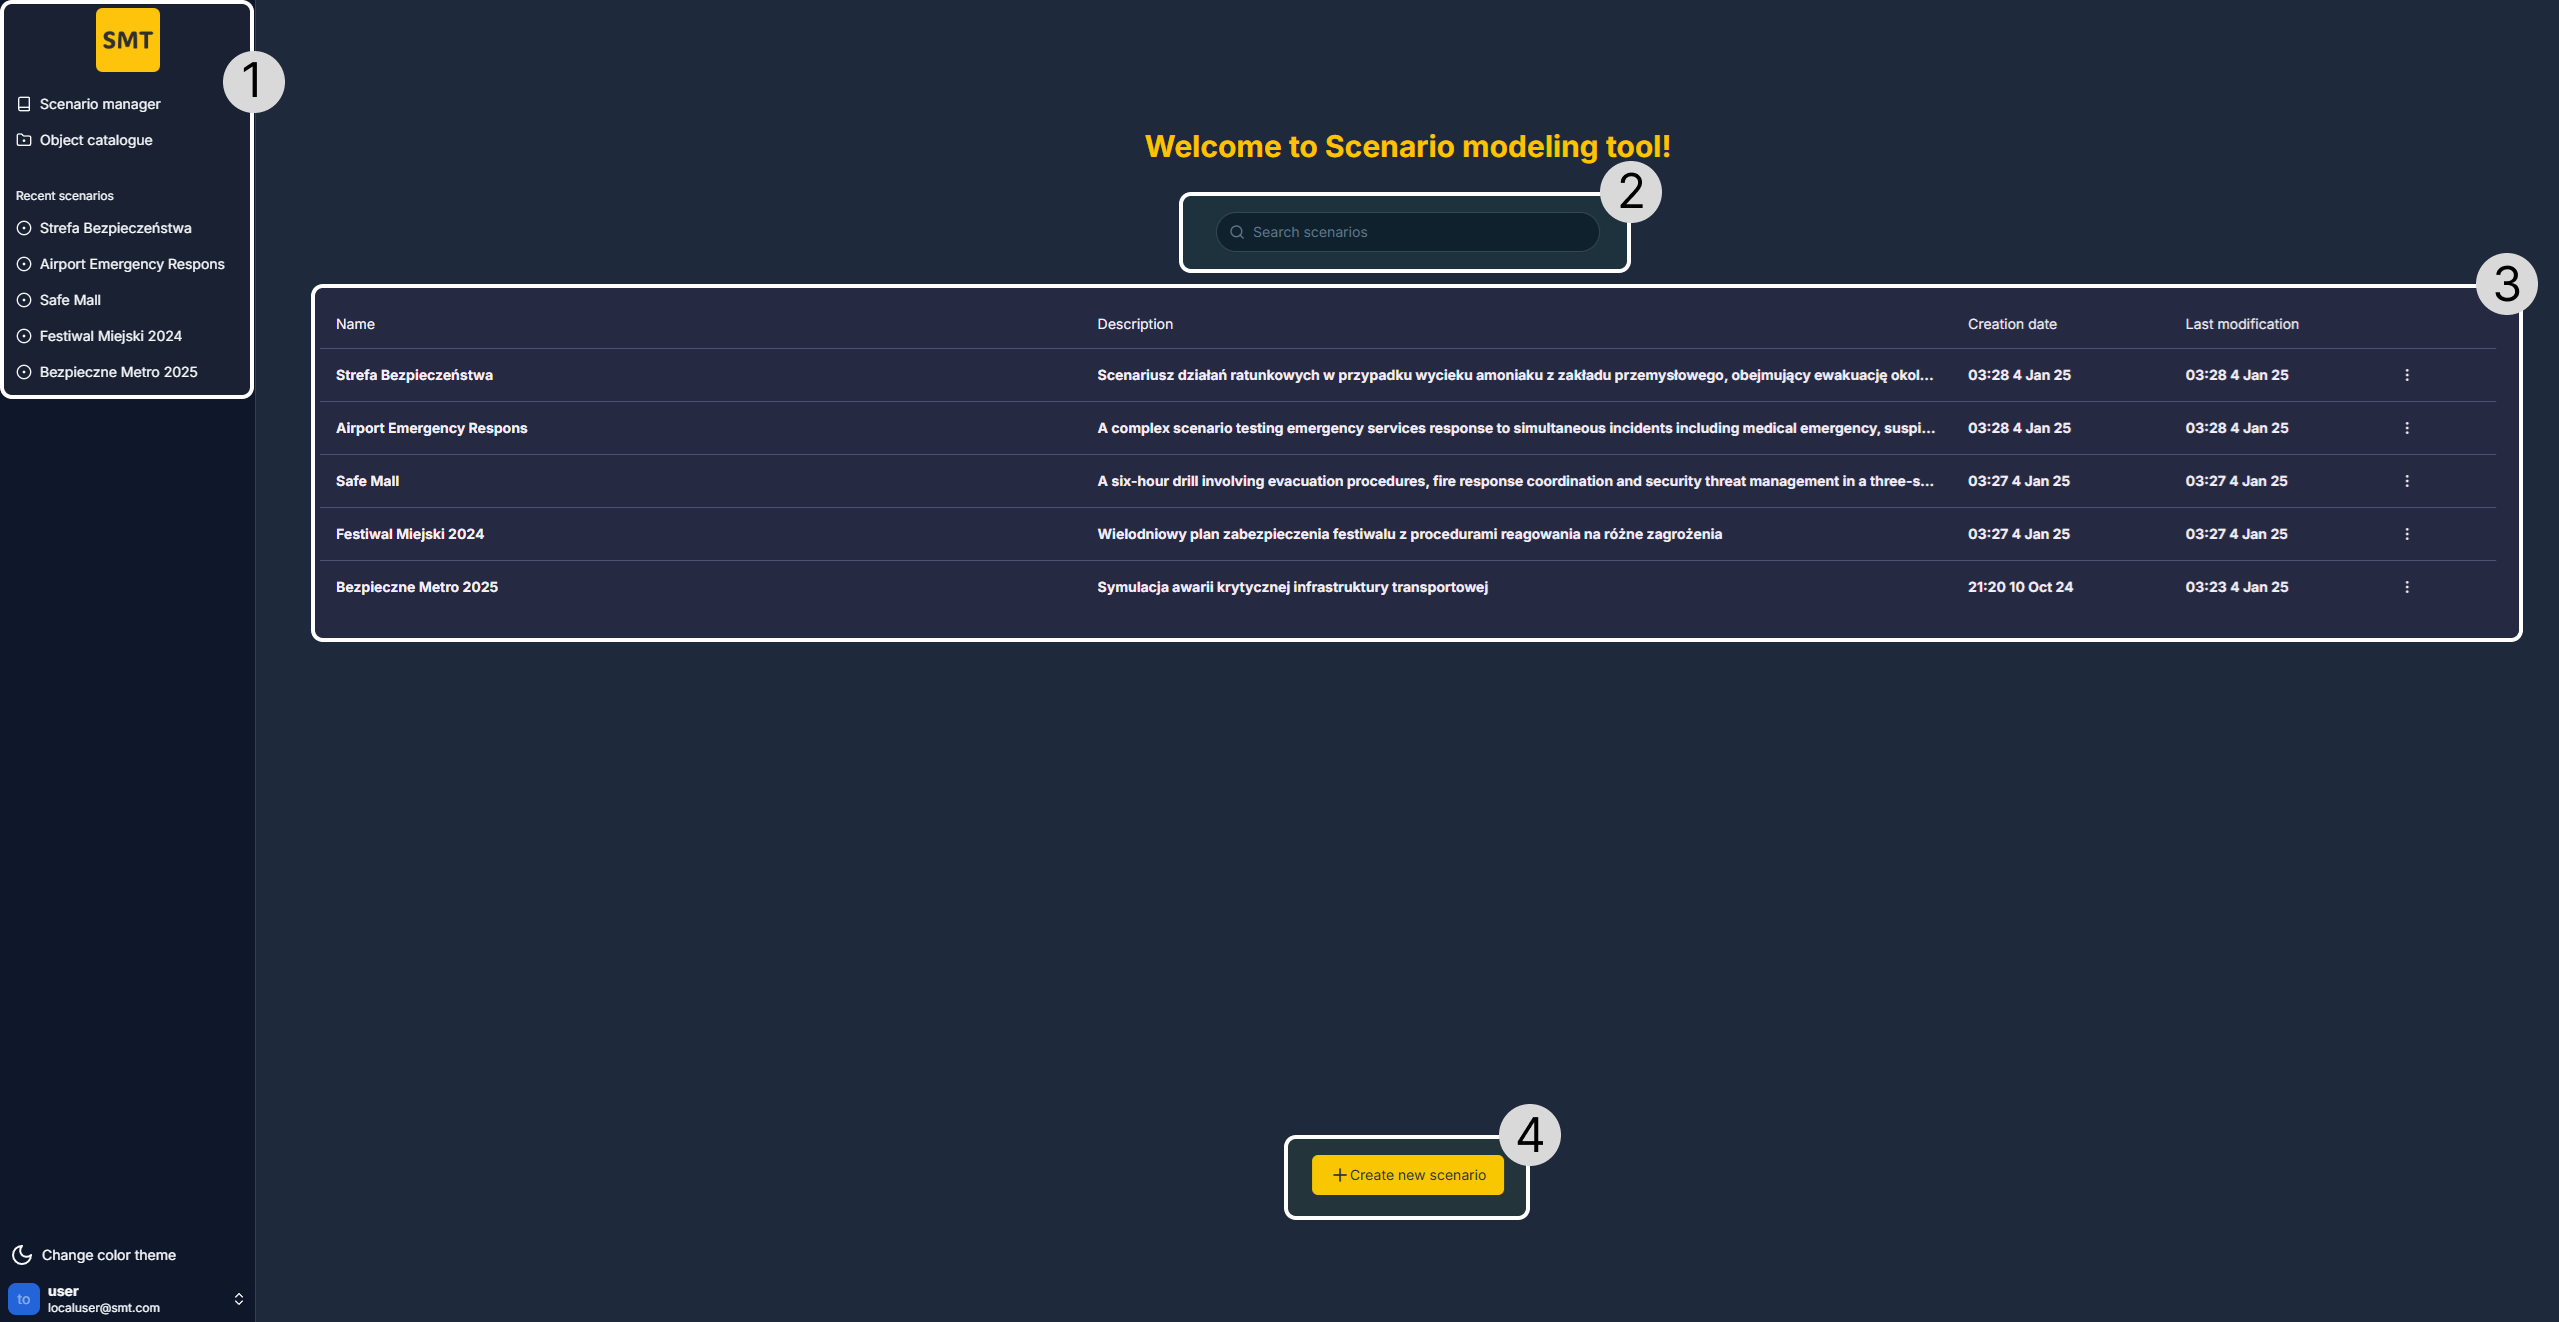
\includegraphics[width=\textwidth]{resources/local/04-implementacja/frontend/landing/landing-page-filled}
    \caption{Widok katalogu scenariuszy}
    \label{fig:scenario_manager}
\end{figure}

Strona ta składa się z czterech głównych elementów funkcjonalnych. 
Panel boczny pełni rolę głównego narzędzia nawigacyjnego systemu, pozwalając na szybkie przełączanie między menedżerem scenariuszy a katalogiem obiektów biblioteki. W jego dolnej części znajduje się sekcja szybkiego dostępu do ostatnio edytowanych scenariuszy oraz panel zarządzania kontem użytkownika.


Centralna część interfejsu zawiera pole wyszukiwania, umożliwiające filtrowanie wyświetlanych scenariuszy w czasie rzeczywistym na podstawie wprowadzanej nazwy. Poniżej znajduje się tabela scenariuszy, prezentująca listę wszystkich dostępnych w systemie scenariuszy.
W dolnej części interfejsu umieszczono przycisk tworzenia nowego scenariusza, który inicjuje proces dodawania nowego scenariusza do systemu.

Posumowując interfejs, ten składa się z następujących elementów:
\begin{enumerate}
    \item Panel boczny z dostępem do funkcji systemu.
    \item Pole wyszukiwania scenariuszy.
    \item Tabela scenariuszy z informacjami o nazwie, opisie i datach modyfikacji.
    \item Przycisk tworzenia nowego scenariusza.
\end{enumerate}

\subsubsection{Tabela scenariuszy}
Tabela prezentuje graficzną reprezentację encji qds\textunderscore scenario, wyświetlając dla każdego scenariusza skrócony tytuł, opis oraz sformatowane daty utworzenia i ostatniej modyfikacji. Po przekroczeniu 10 elementów, aktywuje się system paginacji z nawigacją między stronami wyników.
Interakcja z poszczególnymi scenariuszami możliwa jest poprzez kliknięcie lewym przyciskiem myszy, co prowadzi do edytora scenariusza. Dodatkowe opcje edycji i usunięcia scenariusza dostępne są zarówno przez menu rozwijane z prawej strony wiersza, jak i przez menu kontekstowe wywoływane prawym przyciskiem myszy. Oba menu zawierają identyczny zestaw funkcji.
\begin{figure}[h]
    \centering
    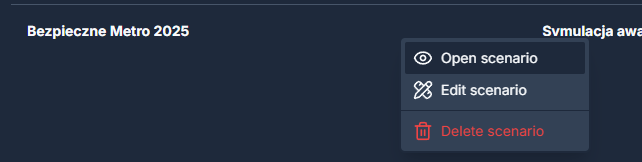
\includegraphics[width=\textwidth]{resources/local/04-implementacja/frontend/landing/context-menu}
    \caption{Menu kontekstowe scenariusza}
\end{figure}

\subsubsection{Formularz tworzenia scenariusza}
\begin{figure}[h]
    \centering
    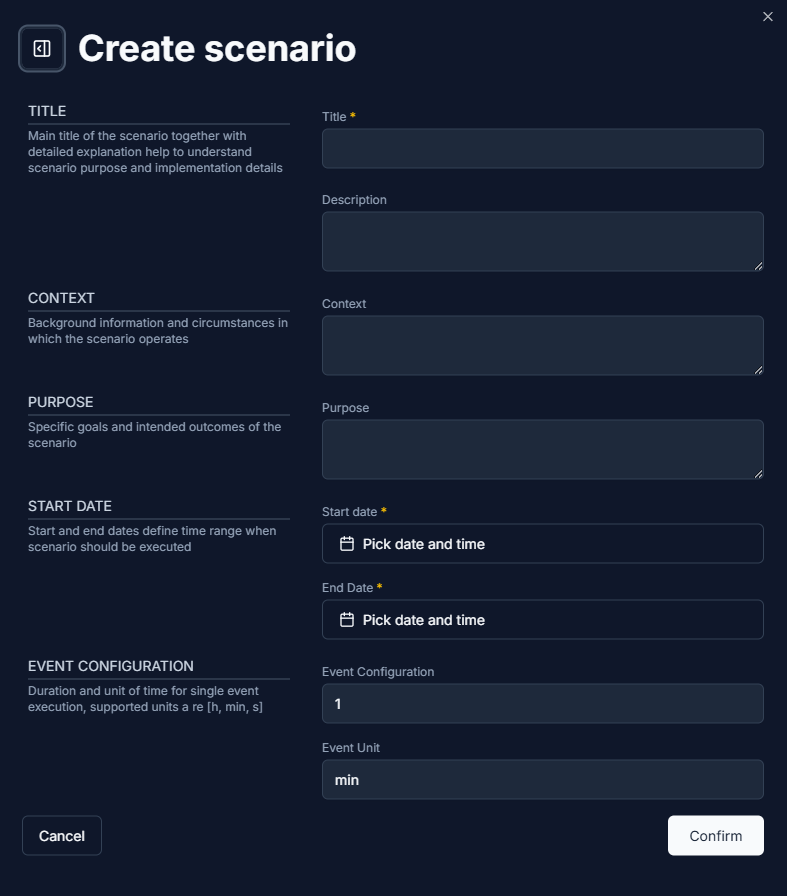
\includegraphics[width=\textwidth]{resources/local/04-implementacja/frontend/landing/create-scenario-form}
    \caption{Rozwinięty formularz tworzenia scenariusza}
    \label{fig:create_scenario}
\end{figure}
Formularz tworzenia nowego scenariusza wyświetlany jest w centralnej części interfejsu, z przyciemnionym tłem aplikacji. Zawiera następujące pola:
\begin{itemize}
    \item Title - główny tytuł scenariusza wraz z opisem szczegółowym (pole wymagane).
    \item Description - opis ogólny scenariusza.
    \item Context - informacje o tle i okolicznościach wykonywania scenariusza.
    \item Purpose - cele i zamierzone rezultaty scenariusza.
    \item Start Date i End Date - zakres czasowy wykonania scenariusza (pola wymagane).
    \item Event Configuration - konfiguracja czasu pojedynczego wydarzenia z wyborem jednostki czasu (h, min, s).
\end{itemize}
W rozwiniętej formie formularza, wszystkie opisy pól widoczne są po lewej stronie interfejsu, dostarczając szczegółowych informacji o przeznaczeniu każdego pola.
System Event Configuration pozwala na wybór jednostki czasu (h, min, s) dla pojedynczego wydarzenia. Domyślnie dostępna jest dowolna jednostka, jednak wybór konkretnej jednostki (godziny, minuty lub sekundy) udostępnia dodatkowe opcje konfiguracji specyficzne dla danej jednostki czasu.
Po wypełnieniu formularza dane przesyłane są do backendu poprzez interfejs REST API. Formularz implementuje wstępną walidację danych - przykładowo, jeśli data rozpoczęcia jest późniejsza niż data zakończenia, pod polem Start Date wyświetlany jest komunikat o niemożliwej konfiguracji. W przypadku poprawnej walidacji i pomyślnej odpowiedzi z serwera, formularz zostaje zamknięty, wyświetlane jest powiadomienie o sukcesie, a nowy scenariusz pojawia się na liście. W przypadku błędu zwróconego przez API, system wyświetla odpowiedni komunikat błędu.
Zamknięcie formularza możliwe jest poprzez kliknięcie poza jego obszarem, użycie przycisku Cancel lub klawisza Escape. Zatwierdzenie formularza następuje po kliknięciu przycisku Confirm lub użyciu klawisza Enter.

\subsubsection{Dialog usuwania scenariusza}
\begin{figure}[h]
    \centering
    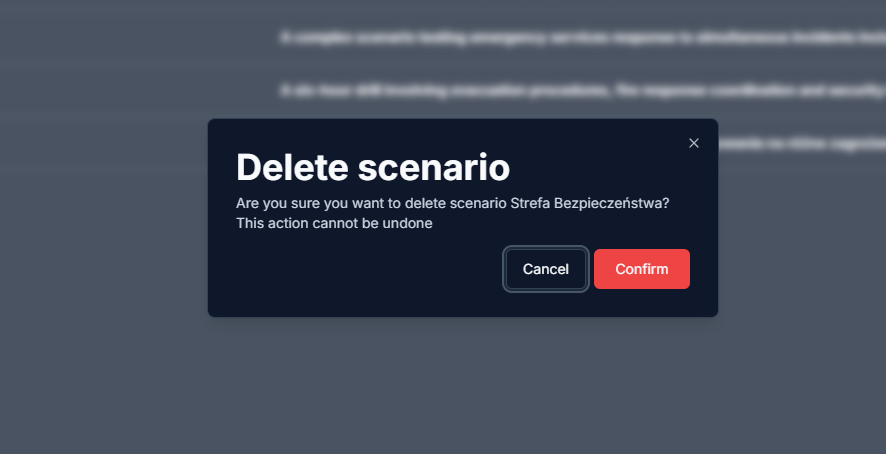
\includegraphics[width=\textwidth]{resources/local/04-implementacja/frontend/landing/delete-scenario-form}
    \caption{Dialog potwierdzenia usunięcia scenariusza}
    \label{fig:delete_scenario}
\end{figure}
Dialog potwierdzenia usunięcia scenariusza wyświetlany jest po wybraniu opcji usunięcia z menu kontekstowego lub rozwijanego. Zawiera on informację ostrzegawczą o nieodwracalności operacji wraz z nazwą usuwanego scenariusza oraz przyciski Cancel i Confirm.
Po zatwierdzeniu, wysyłane jest żądanie do API, a użytkownik informowany jest o statusie operacji poprzez system powiadomień. Podobnie jak w przypadku innych formularzy, dialog można zamknąć poprzez kliknięcie poza jego obszarem, użycie przycisku Cancel lub klawisza Escape.
